\documentclass[11pt]{article}
\usepackage[margin=1in]{geometry}
\usepackage{amsmath,amssymb,amsthm}
\usepackage{booktabs,tabularx,array}
\usepackage{graphicx}
\usepackage[hidelinks]{hyperref}
\usepackage{enumitem}
\setlist{itemsep=2pt,topsep=4pt}

\newtheorem{theorem}{Theorem}
\newtheorem{proposition}[theorem]{Proposition}
\newtheorem{corollary}[theorem]{Corollary}
\theoremstyle{definition}
\newtheorem{definition}[theorem]{Definition}
\newtheorem{observation}[theorem]{Observation}
\newtheorem{counterexample}[theorem]{Counterexample}
\theoremstyle{remark}
\newtheorem{remark}[theorem]{Remark}

\newcommand{\Z}{\mathbb{Z}}
\newcommand{\CF}{\mathrm{CF}}
\newcommand{\NCF}{\mathrm{NCF}}
\newcommand{\lmin}{\ell_{\min}}
\newcommand{\one}{\mathbf{1}}

\title{Loop holonomy under noise:\\ invariants of lossy operation systems at three layers}
\author{}
\date{}

\begin{document}
\maketitle

\begin{abstract}
We replace the group-valued operations of an operation system $(\Gamma,A,g)$ by lossy channels and follow the holonomy through the three layers of the stratification. For shift-covariant uniform noise of rate $\varepsilon$ we prove the following.
\begin{itemize}
  \item The loop operator has character eigenvalues $(1-\varepsilon)^{|L|}\chi(h)$: the modulus records the loss and the phase records the holonomy exactly for every $\varepsilon<1$.
  \item Every per-context Shannon functional, and the loop-composite information, is independent of the holonomy.
  \item On the edge-context empirical model of a single cycle, the contextual fraction is $\max(0,1-|L|\varepsilon/2)$, independent of $|A|$ and of the holonomy.
\end{itemize}
On a general graph we prove $\CF\ge\max(0,1-\lmin\varepsilon/2)$, where $\lmin$ is the length of the shortest cycle with nonzero holonomy, and we observe equality in 44 configurations. Information functionals do not determine the contextual fraction; we give counterexamples. The three layers respond to the same noise through different invariants, and no invariant of one layer determines another.
\end{abstract}

\section{Setting}

Let $\Gamma=(V,E)$ be a finite connected graph and $A$ a finite abelian group of order $n$. Each edge $(a,b)$ carries a doubly stochastic matrix $K_{ab}\in\mathbb{R}^{A\times A}$, where row $x$ is the law of the colour at $b$ given colour $x$ at $a$. Colours are uniform at every vertex, and uniformity is preserved by doubly stochastic channels. Hence the Bayesian inverse of $K_{ab}$ is exactly $K_{ab}^{\top}$, and a loop may be traversed in either direction.

\begin{definition}[Noisy shift]
For $g\in A$ let $S_g$ be the permutation matrix of $x\mapsto x+g$ and $U=\tfrac1n\one\one^{\top}$. The \emph{noisy shift} of rate $\varepsilon\in[0,1]$ is
\[
K=(1-\varepsilon)\,S_g+\varepsilon\,U .
\]
More generally, a \emph{covariant} channel is $K=C_\mu S_g$, where $C_\mu[x,y]=\mu(y-x)$ is convolution by a probability measure $\mu$ on $A$.
\end{definition}

\begin{definition}[Loop operator, edge-context model]
For a closed walk $L=(v_0,v_1,\dots,v_{|L|}=v_0)$, the \emph{loop operator} is $M_L=\prod_{j} K_{v_jv_{j+1}}$, using $K^{\top}$ on edges traversed against their orientation. The \emph{edge-context model} $e_K$ has one measurement per vertex (its colour), one context per edge, and law $\tfrac1n K_{ab}$ on context $(a,b)$.
\end{definition}

By double stochasticity, $e_K$ is no-signalling. At $\varepsilon=0$ it is the all-versus-nothing model $e_g$ of the operation system: its support is the solution set of the linear equations $c_b-c_a=g_{ab}$ over $A$ \cite{abkm15}. We measure contextuality by the contextual fraction $\CF$ \cite{abm17} and by the \v{C}ech obstruction $\gamma$ \cite{amb12}, and we write $\NCF=1-\CF$. For characters $\chi\in\widehat A$ we write $\hat\mu(\chi)=\sum_z\mu(z)\chi(z)$.

\section{Layer 1: the loop operator}

\begin{proposition}[Character eigenvalues]\label{prop:eig}
Let every edge of a simple cycle $L$, oriented along the cycle, carry a covariant channel $C_{\mu_e}S_{g_e}$, and let $h=\sum_e g_e$. Then every character $\chi$ is an eigenvector of $M_L$ with eigenvalue
\[
\lambda_\chi=\Big(\prod_{e\in L}\hat\mu_e(\chi)\Big)\,\chi(h).
\]
For the noisy shift, $M_L=(1-\varepsilon)^{|L|}S_h+\big[1-(1-\varepsilon)^{|L|}\big]U$, so $\lambda_{\mathbf 1}=1$ and $\lambda_\chi=(1-\varepsilon)^{|L|}\chi(h)$ for $\chi\neq\mathbf 1$.
\end{proposition}
\begin{proof}
First, $(S_g\chi)(x)=\chi(x+g)=\chi(g)\chi(x)$. Second, $(C_\mu\chi)(x)=\sum_y\mu(y-x)\chi(y)=\hat\mu(\chi)\chi(x)$. All factors are therefore diagonal in the character basis, so they commute and the eigenvalues multiply. For the noisy shift, $\hat\mu(\chi)=1-\varepsilon$ for $\chi\ne\mathbf 1$, and $S_gU=US_g=U$.
\end{proof}

\begin{corollary}\label{cor:phase}
The labelled eigenvalue $\lambda_\chi$ is independent of the base point of the loop. If every $\hat\mu_e(\chi)$ is real and positive (for instance, symmetric noise with nonvanishing Fourier coefficients), then $\arg\lambda_\chi=\arg\chi(h)$. For the noisy shift, $h$ is recovered exactly for all $\varepsilon<1$.
\end{corollary}

\begin{remark}[What the plain spectrum sees]
The multiset of eigenvalues of $M_L$ is base-point free for \emph{any} channels, since $AB$ and $BA$ share their nonzero spectrum. It does not determine $h$. For the noisy shift on $\Z/n$ it equals $\{1\}\cup\{(1-\varepsilon)^{|L|}e^{2\pi i kh/n}:k\neq0\}$, which depends on $h$ only through its order; on $\Z/5$ every $h\neq0$ gives the same multiset. For asymmetric noise the phase is contaminated. With $\mu=(0.7,0.2,0,0,0.1)$ on $\Z/5$ and $h=2$, the readout is $2.285$, offset by the noise-only phase $0.285$.
\end{remark}

\section{Layer 2: information is blind to the holonomy}

\begin{proposition}\label{prop:blind}
Let $F$ be any functional of a context law that is invariant under relabelling the outcomes of each variable; every Shannon functional is of this kind. Then $F$ takes the same value on $\tfrac1nN S_g$ for every $g$ and every doubly stochastic $N$. In particular, per-edge information never depends on $g$, whether the channel is invertible or lossy.
\end{proposition}
\begin{proof}
Right multiplication by $S_g$ relabels the values of the second variable.
\end{proof}

\begin{proposition}[Closed forms]\label{prop:info}
For the noisy shift and uniform input,
\[
I(c_a;c_b)=\log_2 n+\Big(1-\varepsilon+\tfrac{\varepsilon}{n}\Big)\log_2\Big(1-\varepsilon+\tfrac{\varepsilon}{n}\Big)+(n-1)\tfrac{\varepsilon}{n}\log_2\tfrac{\varepsilon}{n}.
\]
The loop-composite information $I(X;M_LX)$ is given by the same expression with $\varepsilon$ replaced by $\varepsilon_L=1-(1-\varepsilon)^{|L|}$. Both are independent of $h$.
\end{proposition}
\begin{proof}
Each row of $K$ puts mass $1-\varepsilon+\varepsilon/n$ on one colour and $\varepsilon/n$ on each of the other $n-1$. The loop case follows from Proposition~\ref{prop:eig}.
\end{proof}

\begin{table}[h]
\centering
\begin{tabular}{rrrrr}
\toprule
$\varepsilon$ & $I$ edge & $I$ loop, $|L|=3$ & $|\lambda_\chi|$, $|L|=3$ & $\CF$, $\lmin=3$\\
\midrule
0    & 2.3219 & 2.3219 & 1.0000 & 1.000\\
0.05 & 1.9996 & 1.5816 & 0.8574 & 0.925\\
0.10 & 1.7597 & 1.1340 & 0.7290 & 0.850\\
0.20 & 1.3676 & 0.5761 & 0.5120 & 0.700\\
0.30 & 1.0469 & 0.2726 & 0.3430 & 0.550\\
0.50 & 0.5510 & 0.0406 & 0.1250 & 0.250\\
\bottomrule
\end{tabular}
\caption{Noisy shift on $\Z/5$ (information in bits). The information columns are identical for flat and non-flat systems.}
\label{tab:values}
\end{table}

\section{Layer 3: the contextual fraction}

For a colouring $c:V\to A$ and an edge $e=(a,b)$, write $d_e(c)=c(b)-c(a)-g_e$ for its \emph{discrepancy}. Around a cycle $L$ oriented along its edges, $\sum_{e\in L}d_e(c)=-h_L$.

The cells of context $e$ split into discrepancy classes. The class $d=0$ has total mass $1-\varepsilon+\varepsilon/n$, and each class $d\ne0$ has total mass $\varepsilon/n$, spread evenly over its $n$ cells.

\begin{theorem}[Single cycle]\label{thm:cycle}
Let $\Gamma$ be a cycle of length $L\ge3$ with noisy shifts of rate $\varepsilon$ and holonomy $h\neq0$ in a finite abelian group $A$. Then
\[
\CF(e_K)=\max\!\Big(0,\;1-\frac{L\varepsilon}{2}\Big).
\]
In particular, the threshold $\varepsilon^*=2/L$ is independent of $|A|$ and of $h$.
\end{theorem}

\begin{proof}
\emph{Upper bound on $\NCF$.} The non-contextual fraction is the value of the LP $\max\sum_c b_c$ subject to $b\ge0$ and $\sum_{c:\,c|_e=s}b_c\le e_K(e,s)$ for every edge $e$ and section $s$. A feasible point of its dual is a weight $y_e(s)\ge0$ with $\sum_e y_e(c|_e)\ge1$ for every colouring $c$. Take $y_e(s)=w(d)$, where $d$ is the discrepancy of $s$ and
\[
w(0)=0,\qquad w(-h)=1,\qquad w(d)=\tfrac12\ \text{otherwise}.
\]
Every colouring has at least one nonzero discrepancy, since they sum to $-h\neq0$. If it has exactly one, that one equals $-h$ and contributes $1$. Otherwise at least two nonzero discrepancies contribute at least $\tfrac12$ each. So the weight is feasible, and its value is
\[
L\Big[\tfrac{\varepsilon}{n}\cdot1+(n-2)\tfrac{\varepsilon}{n}\cdot\tfrac12\Big]=\frac{L\varepsilon}{2},
\]
so $\NCF\le L\varepsilon/2$.

\emph{Lower bound on $\NCF$ (packing).} Assume $L\varepsilon/2\le1$. A colouring is fixed by its discrepancy vector (summing to $-h$) together with $c(v_0)$. Use two families, each spread uniformly over $c(v_0)\in A$:
\begin{itemize}
  \item[(A)] for each edge $k$, discrepancy $-h$ on $k$ and $0$ elsewhere, with mass $\varepsilon/n$;
  \item[(B)] for each ordered pair of distinct edges $(k,l)$ and each $a\notin\{0,-h\}$, discrepancies $a$ on $k$ and $-h-a$ on $l$, with mass $\beta=\varepsilon/\big(2n(L-1)\big)$.
\end{itemize}
Family (A) uses exactly the mass $\varepsilon/n$ of class $-h$ on each edge. For $a\notin\{0,-h\}$, class $a$ on edge $k$ is used by the triples $(k,l,a)$ and $(l,k,-h-a)$, which is $2(L-1)\beta=\varepsilon/n$, again exactly its mass. Uniform spreading over $c(v_0)$ spreads each class evenly over its $n$ cells, so every off-graph cell is filled to capacity and not beyond.

The total mass is $L\tfrac{\varepsilon}{n}+L(L-1)(n-2)\beta=\tfrac{L\varepsilon}{2}$. On each edge the on-graph cells receive $\tfrac{L\varepsilon}{2}-\varepsilon\big(1-\tfrac1n\big)$, while their capacity is $1-\varepsilon\big(1-\tfrac1n\big)$. The capacity constraint is therefore equivalent to $L\varepsilon/2\le1$, and it is tight exactly at $\varepsilon=2/L$.

\emph{Beyond the threshold.} The model is affine in $\varepsilon$. It is non-contextual at $\varepsilon=2/L$ (just shown) and at $\varepsilon=1$ (a product of uniform laws). Since the non-contextual set is convex, it is non-contextual on the whole interval between them.
\end{proof}

\begin{remark}
For $n=2$, Theorem~\ref{thm:cycle} is the chained Bell inequality \cite{bc90}. The certificate was also checked exhaustively over all colourings for $(n,L,h)\in\{(2,3,1),(3,4,2),(5,3,2),(5,4,1),(4,3,2)\}$. The LP agrees with the formula for $n\in\{2,3,5\}$, $L=3,\dots,6$, and for $A\in\{\Z/2\times\Z/2,\ \Z/2\times\Z/4,\ \Z/3\times\Z/3\}$.
\end{remark}

\begin{theorem}[Any graph, lower bound]\label{thm:graph}
For noisy shifts on any finite connected graph with nonzero class,
\[
\CF(e_K)\ \ge\ \max\!\Big(0,\;1-\frac{\lmin\varepsilon}{2}\Big),
\]
where $\lmin$ is the length of the shortest simple cycle with nonzero holonomy.
\end{theorem}
\begin{proof}
Apply the dual certificate of Theorem~\ref{thm:cycle} on the edges of a shortest non-flat cycle, with weight $0$ elsewhere. Every colouring of $\Gamma$ restricts to a colouring of that cycle, whose discrepancies (signed along the cycle) sum to its nonzero holonomy.
\end{proof}

\begin{observation}[Equality, measured]\label{obs:equality}
Equality holds in Theorem~\ref{thm:graph} in all 44 configurations tested, for $\varepsilon$ up to $0.8$. These cover $\theta$-graphs $\theta(2,3,4)$, $\theta(3,3,3)$, $\theta(1,4,4)$ and $\theta(2,2,5)$; $K_4$; two cycles sharing an edge; two cycles sharing a vertex; and two triangles joined by a path. Only $\lmin$ matters, not the cycle basis. In $\theta(2,2,5)$ with the $4$-cycle flat and only the $7$-cycles non-flat, the slope is $7/2$. A proof of the matching packing on general graphs is open.
\end{observation}

\begin{remark}[$\gamma$]
For every $\varepsilon>0$ the support of $e_K$ is full, so $\gamma=0$. At $\varepsilon=0$, $\gamma(s)\ne0$ for every section over every nonzero coefficient ring, because each context's support is the graph of a bijection.
\end{remark}

\section{What does not hold}

\begin{counterexample}[Information does not determine $\CF$]\label{ce:info}
Consider a $3$-cycle and a $5$-cycle, each with noisy shifts at $\varepsilon=0.2$ over $\Z/3$ and holonomy $1$. Every edge has the same information, yet $\CF=0.70$ and $0.50$.
\end{counterexample}

\begin{counterexample}[Non-covariant noise]\label{ce:noncov}
Let $K_e=\big((1-\varepsilon)I+\varepsilon N_e\big)S_{g_e}$, where $N_e$ is a random mixture of permutations. Then flat systems are already contextual, with $\CF$ up to $0.24$ over $40$ random noise draws at $\varepsilon\in\{0.2,0.5\}$ on a $4$-cycle over $\Z/5$. The phase readout of $h=2$ ranges over $[1.1,3.1]$. Noise and holonomy are no longer separable.
\end{counterexample}

\begin{counterexample}[Entropy is not a function of Fourier moduli]\label{ce:homometric}
Take $p=a*b$ and $q=a*\tilde b$ with $\tilde b(x)=b(-x)$ on $\Z/7$. They have identical $|\hat p|=|\hat q|$, but $H(p)=2.7714$ and $H(q)=2.7689$ bits. The statement ``information depends only on $|\lambda_\chi|$'' holds for the uniform-noise family and not in general.
\end{counterexample}

\section{Summary}

\begin{table}[h]
\centering
\begin{tabularx}{\linewidth}{@{}l>{\raggedright}X>{\raggedright}X l@{}}
\toprule
Layer & Invariant & Response to $\varepsilon$ & Detects $h$ until\\
\midrule
1 Operations & labelled eigenvalue $\lambda_\chi$ of $M_L$ & modulus $(1-\varepsilon)^{|L|}$, phase unchanged & $\varepsilon\to1$\\
2 Probability & per-edge and loop $I$ & decreases, independent of $h$ & never\\
3 Outcomes & $\CF$ & $1-\lmin\varepsilon/2$ & $\varepsilon=2/\lmin$\\
3 Outcomes & $\gamma$ & support becomes full & $\varepsilon=0$ only\\
\bottomrule
\end{tabularx}
\caption{The same noise acting on three invariants.}
\label{tab:robust}
\end{table}

For shift-covariant uniform noise, the modulus of the loop operator's character eigenvalues determines every Shannon functional of the loop channel, and the phase determines $h$. Per-context and loop-composite information are independent of $h$. The contextual fraction is certified by an LP dual and is not determined by information functionals. The labelled phase detects $h$ for every $\varepsilon<1$, including $\varepsilon\ge2/\lmin$, where $\CF=0$. The layers are therefore separated under noise, not bridged.

\begin{figure}[h]
\centering
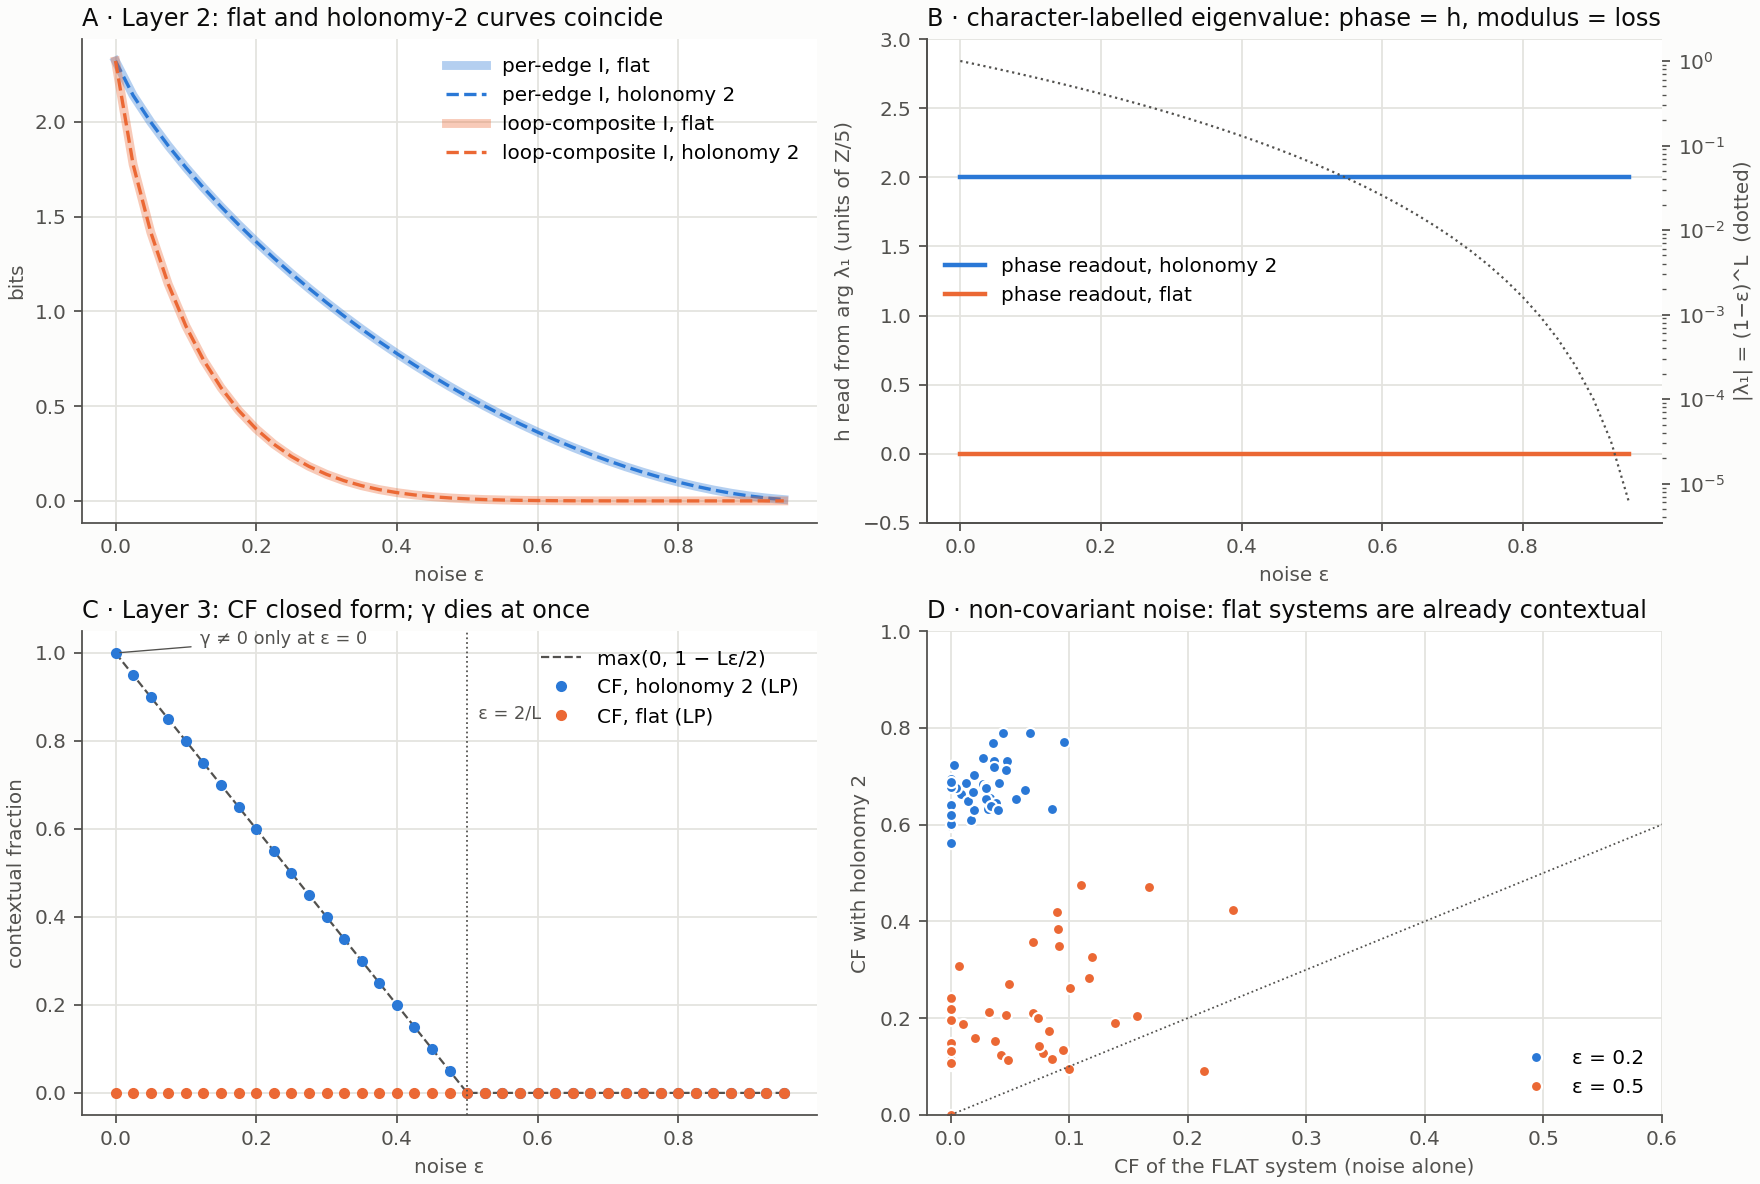
\includegraphics[width=\linewidth]{channels.png}
\caption{A $4$-cycle over $\Z/5$ with $h=2$, compared with a flat system.
(A) Per-edge and loop information coincide for the two systems.
(B) The labelled phase reads $h=2$ while the modulus decays as $(1-\varepsilon)^4$.
(C) $\CF$ follows $\max(0,1-L\varepsilon/2)$; the flat system has $\CF=0$.
(D) Under non-covariant noise, flat systems are already contextual.}
\label{fig:channels}
\end{figure}

\section{Corrections to the previous draft}
\begin{enumerate}
  \item \emph{Attribution.} No ``Brunner--Bergh--Gisin--Vertesi'' framework could be identified. The Layer~3 geometry is that of the local polytope \cite{brunner14}, the contextual fraction \cite{abm17} and sheaf contextuality \cite{ab11}. Vigneaux's framework \cite{vigneaux19,bb15} is information cohomology on sites where every set of observables has a joint; the contextuality statements here are not his.
  \item \emph{Information formula.} The two-point form $\log_2 n+(1-\varepsilon)\log_2(1-\varepsilon)+\varepsilon\log_2(\varepsilon/n)$ is replaced by Proposition~\ref{prop:info}. At $n=5$, $\varepsilon=0.2$ the old form gives $1.1356$; the correct value is $1.3676$.
  \item \emph{Conditional entropy.} The earlier expression gave $3.51>\log_2 5$ bits, which is impossible. The correct value is $H=\log_2 n-I$.
  \item \emph{``Information bounds dictate $\CF$''} is false (Counterexample~\ref{ce:info}).
  \item \emph{``Entropies depend on singular values or on $|\lambda|$''} is false in general (Counterexample~\ref{ce:homometric}).
  \item \emph{``The spectrum reads $h$''} becomes the labelled eigenvalue (Corollary~\ref{cor:phase}); the multiset sees only the order of $h$.
  \item \emph{Spectral bridge.} The phase survives beyond $\CF=0$, which is a separation, not a bridge.
  \item \emph{Threshold.} $\varepsilon^*=2/|L|$ becomes $2/\lmin$ on general graphs: proved as a bound, observed as equality.
  \item \emph{Loop joint.} The loop joint $P(X_0,X_L)$ is a law derived from composing channels, not a section of an information structure.
\end{enumerate}

\section{Open problems}
\begin{enumerate}
  \item Prove equality in Theorem~\ref{thm:graph}, by extending the cycle packing to general graphs.
  \item Find an invariant for non-covariant noise that separates the noise from the holonomy.
  \item Estimate $\lambda_\chi$ from edge readings: which observation designs make the phase identifiable, and at what sample cost? This links the present results to Problem~26.
\end{enumerate}

\paragraph{Reproduction.} All statements are checked by \texttt{tests/test\_channels.py} (81 tests pass in total). The figure is produced by \texttt{examples/channels.py}. The functions are \texttt{noisy\_shift\_information}, \texttt{loop\_information}, \texttt{cf\_noisy\_cycle}, \texttt{cf\_noisy\_graph}, \texttt{holonomy\_girth} and \texttt{character\_value} in \texttt{amb\_vigneaux/channels.py}.

\begin{thebibliography}{9}
\bibitem{ab11} S.~Abramsky and A.~Brandenburger. The sheaf-theoretic structure of non-locality and contextuality. \emph{New J.\ Phys.} 13:113036, 2011.
\bibitem{amb12} S.~Abramsky, S.~Mansfield, and R.~S.~Barbosa. The cohomology of non-locality and contextuality. \emph{EPTCS} 95:1--14, 2012.
\bibitem{abkm15} S.~Abramsky, R.~S.~Barbosa, K.~Kishida, R.~Lal, and S.~Mansfield. Contextuality, cohomology and paradox. In \emph{CSL 2015}, LIPIcs 41, 2015.
\bibitem{abm17} S.~Abramsky, R.~S.~Barbosa, and S.~Mansfield. Contextual fraction as a measure of contextuality. \emph{Phys.\ Rev.\ Lett.} 119:050504, 2017.
\bibitem{brunner14} N.~Brunner, D.~Cavalcanti, S.~Pironio, V.~Scarani, and S.~Wehner. Bell nonlocality. \emph{Rev.\ Mod.\ Phys.} 86:419, 2014.
\bibitem{bc90} S.~L.~Braunstein and C.~M.~Caves. Wringing out better Bell inequalities. \emph{Ann.\ Phys.} 202:22--56, 1990.
\bibitem{bb15} P.~Baudot and D.~Bennequin. The homological nature of entropy. \emph{Entropy} 17(5):3253--3318, 2015.
\bibitem{vigneaux19} J.~P.~Vigneaux. \emph{Topology of Statistical Systems: A Cohomological Approach to Information Theory}. PhD thesis, Universit\'e Paris Diderot, 2019.
\end{thebibliography}

\end{document}
